\exercise{Spatial filtering}
\subsection*{a - Convolution}
Spatial filtering is an operation where each pixel is changed by the pixel values of a neighborhood. By performing this operation some operations can take place that are not possible with just pointwise operations, such as blurring, sharpening or edge detection. When performing spatial filtering on an image it is normally defined how a pixel is influenced by its neighborhood. These influence factors are also called the kernel or mask. By applying the mask to each pixel a spatial filtered result may be obtained. The best way we could think of to have pixels interact with a mask is by convolution. We have implemented this operation in the following Matlab code: 
\matlabexternal{IPfilter.m}
This function can convolute any image with a mask of any size. To test that it functions correctly we have tried to apply a Gaussian kernel (as in table~\ref{tbl:gauss}) to an image which should blur the original image. Figures~\ref{fig:nonblur} and~\ref{fig:blur} illustrate the correct result.
\begin{figure}[!htb]
 \centering
 \begin{subfigure}[b]{0.49\linewidth}
  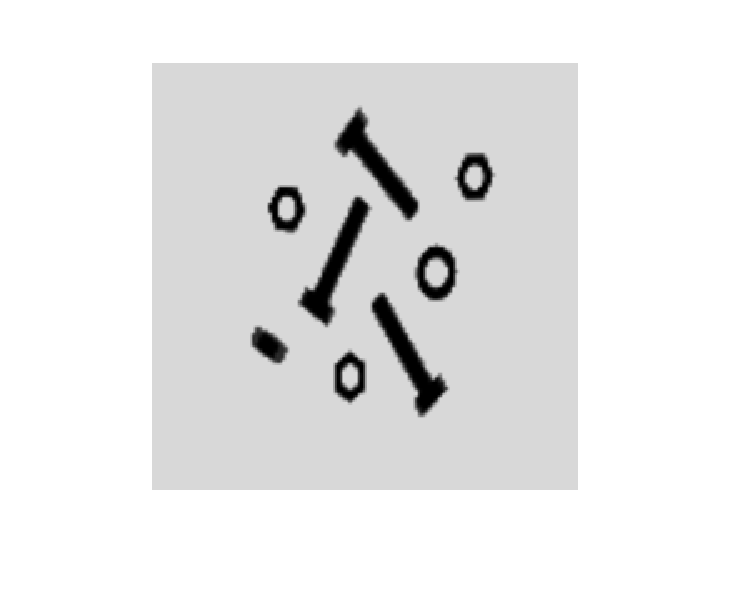
\includegraphics[width=\textwidth]{notBlurred.eps} 
  \caption{An image which was not blurred}
  \label{fig:nonblur} 
 \end{subfigure}
 \begin{subfigure}[b]{0.49\linewidth}
  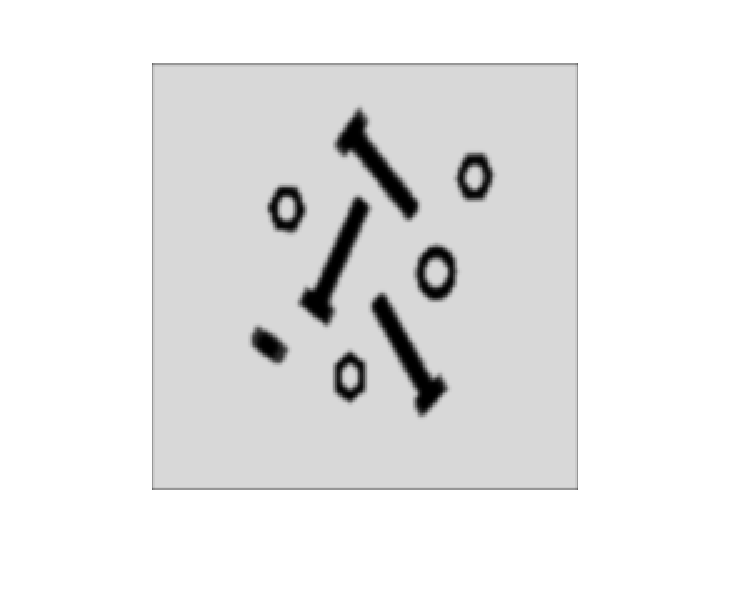
\includegraphics[width=\textwidth]{blurred.eps}
  \caption{The same image convoluted with a Gaussian kernel}
  \label{fig:blur}
 \end{subfigure}
 \caption{Gaussian mask applied to an image to demonstrate convolution}
\end{figure}
\begin{table}[!htb]
\begin{center}
$\frac{1}{273}$
\begin{tabular}{|c|c|c|c|c|}\hline
1 & 4 & 7 & 4 & 1\\ \hline
4 &  16 &  26 &  16 &  4 \\ \hline
7 &  26 &  41 &  26 &  7\\ \hline
4 &  16 &  26 &  16 &  4\\ \hline
1 &  4 &  7 &  4 &  1 \\ \hline
\end{tabular}

\caption{Gaussian kernel for blurring}
\label{tbl:gauss}
\end{center}
\end{table}
